\section{Details of Human Experiments}
\label{app:human_experiment}
\begin{figure}[b]
    \centering
    \begin{subfigure}[t]{0.49\linewidth}
        \centering
        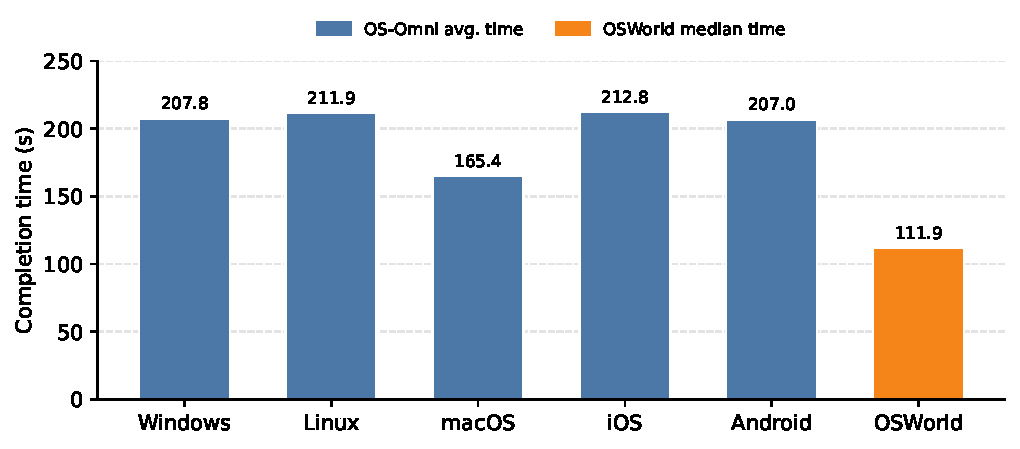
\includegraphics[width=\linewidth]{figures/human_time_comparison.pdf}
        \caption{Human completion time on \dataset by platform. Blue bars report the average completion time for each \dataset platform, and the orange bar shows the OSWorld reported median completion time.}
        \label{fig:human_time_comparison}
    \end{subfigure}
    \hfill
    \begin{subfigure}[t]{0.49\linewidth}
        \centering
        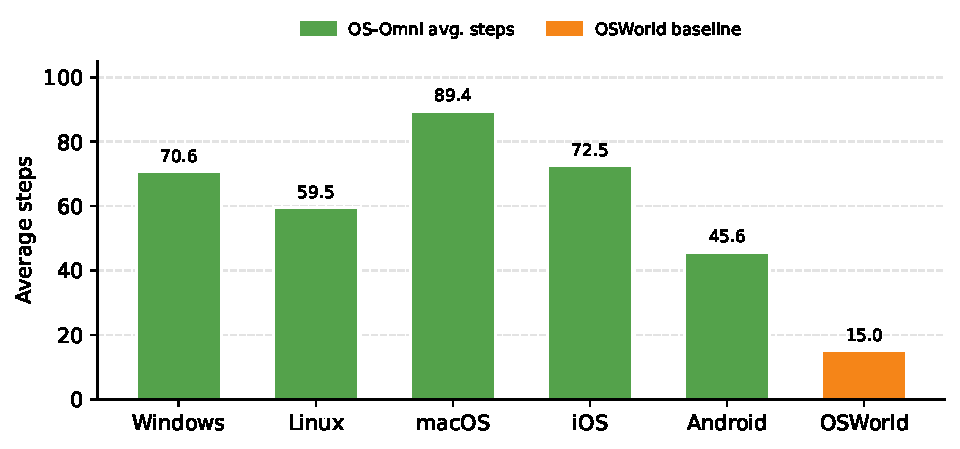
\includegraphics[width=\linewidth]{figures/human_steps_comparison.pdf}
        \caption{Human interaction steps on \dataset by platform. Bars report the average number of interaction steps needed by human annotators on each platform.}
        \label{fig:human_steps_comparison}
    \end{subfigure}
\end{figure}


As shown in Figures~\ref{fig:human_time_comparison} and~\ref{fig:human_steps_comparison}, human users require substantial effort across all \dataset platforms. Averaged over Windows, Linux, macOS, iOS, and Android, a task takes 67.54 interaction steps and 200.97 seconds to complete. This is 1.80$\times$ the OSWorld reported median completion time of 111.94 seconds~\citep{xie2024osworld}. Even the fastest \dataset platform, macOS, takes 165.41 seconds on average, or 1.48$\times$ the OSWorld reference; iOS, Linux, Windows, and Android cluster between 207.00 and 212.79 seconds, corresponding to 1.85--1.90$\times$ the OSWorld time.

The per-platform measurements also show that task burden is not determined by action count alone. Android has the fewest human steps (45.63) but still requires 207.00 seconds on average, while macOS has the most steps (89.43) but the shortest average time among \dataset platforms. This gap indicates that human effort depends on platform-specific feedback latency, application startup and navigation cost, file or state inspection, and the need to verify persistent artifacts, rather than simply the number of GUI actions. OSWorld further reports 72.36\% human accuracy, compared with 88\% on WebArena~\citep{zhou2023webarena}, showing that executable desktop tasks are already harder than pure web tasks. \dataset extends this difficulty to a broader cross-platform setting, where users must handle heterogeneous operating systems, application ecosystems, and state representations.


\section{Details of \textsc{OS-Omni} Environment}
\label{app:osomni_env}

\subsection{Environment Infrastructure}
\label{app:osomni_env_infra}

\textsc{OS-Omni} supports both containerized and non-containerized deployment. The containerized path packages the host-side runner, dependencies, local services, and orchestration logic into a reproducible software environment, which is convenient for headless servers and shared evaluation machines. The non-containerized path runs the same components directly on the host system, which is useful for local development, debugging, and platform-specific runtime control. In both cases, deployment is separated from the environment seen by the agent.

\textsc{OS-Omni} provides runtime support for desktop, mobile, and web endpoints through controlled execution environments. The agent-facing environments are instantiated through platform-specific runtimes, with the host-side components deployed either inside or outside containers. Desktop endpoints are instantiated through managed virtual machines, mobile endpoints are instantiated through emulators or simulators, and web tasks are instantiated through controlled browser environments on the supported operating systems. Ubuntu and Windows are controlled through the desktop runtime interface, macOS through the Apple-platform runtime interface, Android through ADB, iOS through an XCUITest-based automation backend, and web tasks through browser-specific controllers and local benchmark services. This design preserves each platform's native UI stack, application state, and input behavior while keeping the host-side execution stack reproducible.

Across these backends, the runtime layer exposes the same episode contract. It restores or prepares the guest, applies the task initializer, captures observations, executes actions, retrieves artifacts, and invokes the final-state evaluator. Cross-platform tasks are handled by a runner that executes two platform episodes in sequence and transfers the required artifact through the host. Every guest is restored or reset from a clean baseline before each task so that initial state is reproducible, and multiple guests can run in parallel on a single host.

\subsection{Observation Space}
\label{app:osomni_obs}

\textsc{OS-Omni} supports three observation modes through the execution specification: screenshot-only, accessibility-tree-only, and combined screenshot-plus-tree observation. The primary protocol used in the main results is screenshot-only, because screenshots are naturally available across desktop, mobile, web, and cross-platform workflows without assuming that every application exposes clean structured UI metadata. Accessibility-tree-only and combined-observation modes are supported for alternative protocols, debugging, and ablation studies. Some runtime backends can also expose terminal output for command-line workflows, but terminal output is an auxiliary channel rather than a main benchmark observation mode. Trajectory artifacts (per-step screenshots, model responses, controller status, and the final evaluator output) are recorded for post-hoc inspection but are not surfaced to the agent at decision time. \textsc{OS-Omni} supports observation refactoring and extension if needed, such as restricting the observation to a focused application or adding a scoped DOM extract.

\subsubsection{Screenshot}
\label{app:osomni_screenshot}

To align with the perception of a human user, we capture a screenshot of the entire device screen at every step. Including the mouse cursor also proves helpful in certain cases where mouse information is crucial. For desktop resolution, we default to $1920 \times 1080$, which offers a 16:9 aspect ratio and matches the most commonly used desktop resolution in worldwide statistics. On mobile, the screenshot is captured at the device's native resolution. \textsc{OS-Omni} also supports modifying the resolution of virtual machines to avoid potential memorization of absolute pixel values and to assist studies on topics like generalization across different resolutions. Screenshots are persisted under per-episode run directories so that a trajectory can be replayed visually and the final state can be audited independently of the evaluator's structured checks.

\subsubsection{Accessibility Tree}
\label{app:osomni_a11y}

An accessibility tree (or a11y tree) refers to an intricate structure generated by the OS or browser accessibility APIs that renders a representative model of the on-screen content, providing a means of interaction for assistive technologies. Each node within the accessibility tree hosts important information about a UI element. This could range from the nature of the object (a button, checkbox, list item, or paragraph of text), its current state (checked or unchecked, focused or hidden), and even its spatial orientation on the screen.

Different operating systems employ varied accessibility APIs to construct and manipulate the accessibility tree. These include UI Automation (UIA) and Microsoft Active Accessibility (MSAA) for Windows, the NSAccessibility / AX protocol for macOS, the Assistive Technology Service Provider Interface (ATSPI) for the GNOME desktop used on Ubuntu, the device view-hierarchy dump for Android, and XCUITest element trees for iOS. \textsc{OS-Omni} normalizes these per-platform sources into a shared per-node schema that carries an identifier, a type, visible text, a selector, the enabled / focused / active flags, and the on-screen bounding rectangle, so that the same agent interface can address an element by either node identifier or pixel coordinate. Because the information returned by these accessibility APIs differs in coverage and noise level across platforms, we treat structured metadata as a diagnostic and ablation channel rather than as a privileged oracle.

 
\subsubsection{Terminal Output}
\label{app:osomni_terminal}

\textsc{OS-Omni} also supports terminal output as an optional observation channel for command-line workflows. When enabled, the runtime returns the text shown in the active terminal session or the output exposed by the platform command interface, depending on the backend. This channel is useful for tasks involving shell commands, script execution, logs, and text-based tools, where the relevant state may be textual and not fully recoverable from screenshots alone.

Terminal output is not part of the main screenshot-only protocol. We reserve it for compatible environments, debugging, and ablation studies so that the primary reported setting remains aligned with the visual information available across desktop, mobile, web, and cross-platform workflows.

 

\subsection{Action Space}
\label{app:osomni_action}

We implement two kinds of action space: a free-form PyAutoGUI action space, used as the main interface on desktop platforms, and a structured \emph{computer-style} action schema that is exposed by every platform runner and shared across desktop, mobile, and web tasks. The PyAutoGUI action space saves tokens for describing the action space in prompting and matches the OSWorld baselines; the structured schema is finite and parameterized, which makes it more suitable for tool-calling APIs, constrained decoding, and reinforcement-learning-style training. Both interfaces share the same episode lifecycle and the same final-state evaluator, so they are experimental choices rather than separate benchmarks. The terminal symbols \texttt{DONE}, \texttt{FAIL}, and \texttt{WAIT} are common to both interfaces and are the only ways an episode can end other than the per-step or per-episode budget.


\subsubsection{PyAutoGUI}
\label{app:osomni_pyautogui}

\texttt{pyautogui} is an open-source, cross-platform Python module utilized for programmatically controlling the mouse and keyboard. It controls cursor movement, single and multi-button clicks, drags, scroll wheel events, and keyboard input. We adopt PyAutoGUI as our core desktop control component, and we use it as the main agent-facing action space on desktop platforms because it tokenizes compactly, generalizes across Ubuntu/Linux, Windows, and macOS, and matches the style of code used in prior baselines.

At each step, the agent is asked to first give a short reflection on the current screenshot and previous actions, and then to return one fenced Python block that contains the next action(s). Specifically, it may also return one of three special blocks: \texttt{WAIT} when it needs the application to settle, \texttt{FAIL} when it determines the task cannot be performed, or \texttt{DONE} when it determines that the task is complete. The on-guest sandbox only allows \texttt{import pyautogui}, \texttt{import time}, direct \texttt{pyautogui} calls, simple loops, and \texttt{print}; modules such as \texttt{os}, \texttt{subprocess}, or \texttt{tkinter} are not importable, and \texttt{pyautogui.screenshot()} and \texttt{pyautogui.locateCenterOnScreen} are explicitly disallowed. This isolates ``the agent moves the mouse and keyboard'' from ``the agent edits files or runs shell commands,'' so that screenshot-only success cannot be accidentally laundered through an unrelated automation
API.

A representative episode therefore alternates between short natural-language reflections and minimal PyAutoGUI snippets:

\small
\begin{Verbatim}[fontsize=\small]
# step k reflection
The Calc workbook is open on Sheet1 and the cursor is in A1.
I need to enter the SUM formula, so I will click B10 first.

```python
import pyautogui, time
pyautogui.click(x=412, y=638)
time.sleep(0.3)
pyautogui.typewrite("=SUM(B2:B9)", interval=0.02)
pyautogui.press("enter")
```
\end{Verbatim}
\normalsize

\subsubsection{Structured Action Schema}
\label{app:osomni_action_schema}

To facilitate tool-calling APIs and potential reinforcement-learning applications, \textsc{OS-Omni} also exposes a structured variant in which actions are wrapped into a finite class with parameterized enumeration. This structured approach supports constrained decoding by providing a distinct set of actions to be learned and optimized. The schema is shared across desktop, mobile, and web lanes so that the same agent interface covers heterogeneous endpoint types while preserving backend-specific execution. In every case, the \texttt{target} field of a pointing action accepts either an absolute pixel coordinate \texttt{[x,~y]}, a normalized coordinate \texttt{\{"x":~0.5,~"y":~0.5\}}, or, when the accessibility tree is exposed to the agent, a node identifier from that tree. Tables~\ref{tab:osomni_desktop_actions}~and~\ref{tab:osomni_mobile_actions} summarize the main desktop and mobile action schemas.

\begin{table}[ht]
\centering
\caption{Action types and parameters defined in the desktop action schema (Ubuntu/Linux, Windows, and macOS). Each desktop guest exposes the same schema to the agent.}
\label{tab:osomni_desktop_actions}
\small
\setlength{\tabcolsep}{5pt}
\renewcommand{\arraystretch}{1.12}
\begin{tabular}{p{2.4cm}p{4.0cm}p{6.6cm}}
\toprule
Action Type & Parameters & Note \\
\midrule
\texttt{TAP}          & \texttt{target}                                              & Click at the specified element or position. \\
\texttt{DOUBLE\_TAP}  & \texttt{target}                                              & Double-click at the specified element or position. \\
\texttt{RIGHT\_CLICK} & \texttt{target}                                              & Right-click at the specified element or position. \\
\texttt{DRAG}         & \texttt{from\_target}, \texttt{to\_target}, \texttt{duration\_ms} & Drag from one position to another with the left button held. \\
\texttt{SCROLL}       & \texttt{direction}, \texttt{distance}, \texttt{target}       & Scroll up, down, left, or right; optional anchor target. \\
\texttt{TYPE\_TEXT}   & \texttt{text}, \texttt{target}, \texttt{clear\_first}        & Type text, optionally after focusing the target field. \\
\texttt{KEYBOARD}     & \texttt{action}, \texttt{count}                              & Press a single key (\texttt{enter}, \texttt{escape}, \texttt{backspace}, \dots) one or more times. \\
\texttt{HOTKEY}       & \texttt{keys}                                                & Press a keyboard shortcut, e.g. \texttt{[ctrl, c]}. \\
\texttt{WAIT}         & \texttt{ms}                                                  & Wait for the UI to settle. \\
\texttt{DONE}         & \texttt{message}                                             & Decide the task is done. \\
\texttt{FAIL}         & \texttt{message}                                             & Decide the task cannot be performed. \\
\bottomrule
\end{tabular}
\end{table}

\begin{table}[ht]
\centering
\caption{Action types and parameters defined in the mobile action schema. A and I indicate availability on Android and iOS, respectively.}
\label{tab:osomni_mobile_actions}
\small
\setlength{\tabcolsep}{5pt}
\renewcommand{\arraystretch}{1.12}
\begin{tabular}{p{2.4cm}p{1.6cm}p{4.4cm}p{4.6cm}}
\toprule
Action Type & Platform & Parameters & Note \\
\midrule
\texttt{TAP}          & A, I & \texttt{target}                                  & Tap at the specified element or position. \\
\texttt{DOUBLE\_TAP}  & I    & \texttt{target}                                  & Double tap at the specified element or position. \\
\texttt{LONG\_PRESS}  & A, I & \texttt{target}, \texttt{duration\_ms}           & Press and hold the target. \\
\texttt{SWIPE}        & A    & \texttt{from\_target}, \texttt{to\_target}, \texttt{duration\_ms} & Swipe from one position to another. \\
\texttt{DRAG}         & I    & \texttt{from}, \texttt{to}, \texttt{duration\_ms} & Drag from one element/position to another, e.g. to reorder. \\
\texttt{SCROLL}       & A, I & \texttt{direction}, \texttt{distance}, \texttt{target}, \texttt{duration\_ms} & Scroll the screen or specified container. \\
\texttt{TYPE\_TEXT}   & A, I & \texttt{text}, \texttt{target}, \texttt{clear\_first} & Type text, optionally after tapping a target field. \\
\texttt{KEYBOARD}     & A, I & \texttt{action}, \texttt{count}                  & Send a keyboard or system key (\texttt{enter}, \texttt{back}, \texttt{home}, \texttt{escape}, \dots). \\
\texttt{CLIPBOARD}    & I    & \texttt{action}, \texttt{text}                   & Set, get, or paste clipboard content. \\
\texttt{ALERT}        & I    & \texttt{action}                                  & Accept or dismiss a system alert / popup. \\
\texttt{SYSTEM}       & I    & \texttt{action}                                  & System action (\texttt{home}, \texttt{hideKeyboard}). \\
\texttt{LAUNCH\_APP}  & A, I & \texttt{name}                                    & Launch an app by package or bundle identifier. \\
\texttt{WAIT}         & A, I & \texttt{ms}                                      & Wait for the UI to settle. \\
\texttt{DONE}         & A, I & \texttt{message}                                 & Decide the task is done. \\
\texttt{FAIL}         & A, I & \texttt{message}                                 & Decide the task cannot be performed. \\
\bottomrule
\end{tabular}
\end{table}

The desktop schema retains the full mouse, keyboard, and shortcut surface that PyAutoGUI exposes, but presents it as a discrete, parameterized action space with explicit terminal symbols, making the desktop lane directly comparable to the mobile lanes during benchmark reporting. The mobile schemas extend the same conceptual interface with the additional intents that touch UIs require, including \texttt{LONG\_PRESS}, \texttt{SWIPE}, \texttt{ALERT}, \texttt{SYSTEM}, and \texttt{LAUNCH\_APP}.
The terminal actions \texttt{DONE} and \texttt{FAIL}, together with \texttt{WAIT} and the host-side step-budget timeout, are the only ways an episode can end; the evaluator is then invoked on the final environment state, so the agent is not rewarded for imitating any particular action trajectory.

